\documentclass{jlreq}

\usepackage{amsmath}
\usepackage{array}
\usepackage{bm}
\usepackage{caption}
\usepackage{fancyhdr}
\usepackage{float}
\usepackage{graphicx}
\usepackage{listings}
\usepackage{multirow}
\usepackage{physics}
\usepackage{siunitx}
\usepackage{xcolor}

\lstset{
    language=Verilog, % 使用するプログラム言語を指定
    basicstyle=\ttfamily\footnotesize, % フォントの指定
    tabsize=4, % インデント幅
    numbers=left, % 行番号を表示(必要な場合)
    numberstyle=\tiny, % 行番号のスタイル
    frame=single, % ソースコードを枠で囲む(必要な場合)
    breaklines=true, % 長い行を自動的に折り返す
    captionpos=t, % キャプションの位置を上にする
    showstringspaces=false, % 文字列内のスペースを表示しない
    keywordstyle=\color{blue}, % キーワードの色
    commentstyle=\color{green}, % コメントの色
    stringstyle=\color{red}, % 文字列の色
}
\renewcommand{\lstlistingname}{ソースコード}

\numberwithin{equation}{section}

\pagestyle{fancy}
\fancyhf{}
\fancyhead[R]{\thepage}

\begin{document}

\tableofcontents
\clearpage

\section{実験の目的}
ハードウェア記述言語(HDL)を用いた組み合わせ回路や順序回路の設計を通してHDLでの設計手法を学び,
実験でのシミュレーションを行う方法を身につける.

\section{実験器具}
実験に用いた環境を以下に示す.
\begin{description}
	\item[PC] Inspiron 15 3535
	\item[OS] Windows11
	\item[CPU] AMD Ryzen 5 7530U with Radeon Graphics 2.00 GHz
	\item[統合開発環境] Quartus Prime Lite Edition Version 20.1.1
	\item[シミュレータ] ModelSim - Intel FPGA Starter Edition
	\item[FPGAボード] Terasic DE1-SoC
\end{description}

\section{理論}
\subsection{ハードウェア記述言語による論理設計}
幅広い分野で用いられている電子機器には,大規模半導体集積回路(LSI)が数多く搭載されている.
このLSIは回路規模が非常に大きく,回路設計の全てを人手で行うことは現実的ではないため,回路の動作を言語によって記述するハードウェア記述言語(HDL)が
広く用いられる.HDLによる回路設計では,HDLで回路の動作をプログラムのように記述した後,論理合成ツールによりゲート回路に変換する.
論理合成ツールはプログラミングにおけるコンパイラに相当し,設計者が定義した設計制約条件に従って論理回路を最適化する.
HDLの構文はC言語などのプログラミング言語の構文とよく似ているが,多くのプログラミング言語がプログラムの逐次的な動作を記述するのに対し,
HDLでは並列動作を記述できるように考慮されている点で大きく異なる.
本実習ではC言語と記述が似ているVerilog HDLを用いる.

\subsection{FPGA}
FPGAは「現場(Field)でプログラム可能(Programmable)なゲートアレイ(Gate Array)」であり,回路構成を電気的に書き込むことができる.
FPGAはいくつかのロジックエレメント(LE)からなるロジックアレイブロック(LAB)を格子状に配置したデバイスであり,各LABは行列方向のインタコネクト(配線部)と接続している.
インタコネクトの接続経路はプログラム可能になっており,LAB間の接続を自由に変更できる.
LEはルックアップテーブル,プログラム可能レジスタなどで構成されており,それらを書き換えたり
インタコネクトの接続を変更することでFPGAをプログラムする.

\subsection{組み合わせ回路の設計}
図\ref{fig:combinational_logic}のように,入力信号だけで出力信号が決まる論理回路を組み合わせ回路(combinational logic)という.
HDLを用いた設計では,設計者は目的とする組み合わせ回路の動作をHDLによって記述するだけで,論理ゲートをどのように接続するかについては論理合成ツールが自動生成する.
\begin{figure}[H]
	\centering
	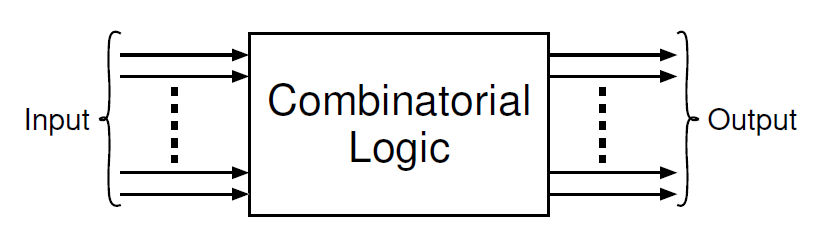
\includegraphics[width=0.7\textwidth]{assets/combinational_logic.png}
	\caption{組み合わせ回路}
	\label{fig:combinational_logic}
\end{figure}

\subsubsection{デコーダ}
デコーダ(decoder)とは入力の組み合わせ(コード)に従って,対応する出力信号を生成する回路である.
$n\text{入力} m(=2^n)\text{出力}$のデコーダを$n \times m$デコーダという.表は,2ビットの入力を4ビットの出力に復号する$2\times4$デコーダの機能表である.
\begin{table}
	\centering
	\caption{$2\times4$デコーダの機能表}
	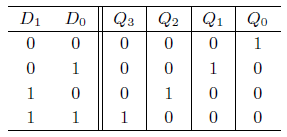
\includegraphics{assets/2x4_decoder_table.png}
	\label{tab:2x4_decoder_function}
\end{table}

\subsubsection{マルチプレクサ}
マルチプレクサ(MUX)とは,複数個の入力値から1個の値を選択して出力する回路である.出力値を選択することからセレクタ(selector)ともいう.
図\ref{fig:2to1_mux}は,1ビットの選択信号Sの値によって2個の1ビット入力X, Yを選択して出力する2-to-1マルチプレクサであり,表\ref{tab:2to1_mux_function}はその機能表である.
\begin{figure}[H]
	\centering
	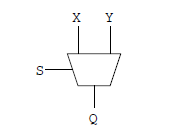
\includegraphics{assets/2to1_mux.png}
	\caption{1ビット2-to-1マルチプレクサ}
	\label{fig:2to1_mux}
\end{figure}

\begin{table}[H]
	\centering
	\caption{1ビット2-to-1マルチプレクサの機能表}
	\begin{tabular}{c|c}
		\hline
		$S$ & $Q$ \\ \hline
		0   & X   \\
		1   & Y   \\ \hline
	\end{tabular}
	\label{tab:2to1_mux_function}
\end{table}

\subsection{順序回路の設計}
順序回路(sequential logic)とは,ある時刻の出力がその時刻での入力と状態(入力履歴)に依存する論理回路である.構成としては,図\ref{fig:sequential_logic}のように
組み合わせ回路に現状態を記憶するメモリを付加したものになる.
\begin{figure}[H]
	\centering
	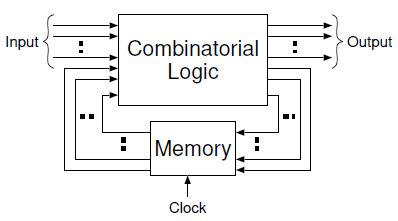
\includegraphics{assets/sequential_logic.png}
	\caption{順序回路}
	\label{fig:sequential_logic}
\end{figure}

順序回路において,動作のタイミングをとる信号をクロック(clock)と呼び,本実習で主に取り扱う同期式順序回路では回路の動作がこのクロックに同期する.
つまり,同期式順序回路ではクロック入力ごとに状態の変化が起こりうるため,クロックごとに順序回路の入力と出力を決定する.

\subsubsection{順序回路における記憶素子}
順序回路の状態を記憶するための機構には, ラッチ(latch)やフリップフロップ(FF)がある.これらは論理値の0または1のいずれかを安定状態として保持する.

\subsubsection{Dフリップフロップ}
ラッチはイネーブル信号が1である間入力を通過させ,イネーブル信号が0になった時に,その時点での入力を記憶する素子である.
図\ref{fig:latch}はラッチを論理ゲートで構成した図である.
\begin{figure}[H]
	\centering
	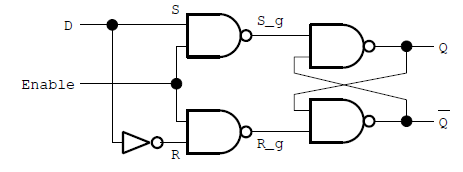
\includegraphics{assets/latch.png}
	\caption{ラッチの回路構成}
	\label{fig:latch}
\end{figure}

ラッチでは,イネーブル信号が1の期間中に入力信号Dが変化すると,Dの変化に連動して即座に出力が変化してしまう.
例えば,図\ref{fig:d-ff_timing}においてClockをイネーブル信号とみなすと,入力Dが変化することで,Q1のような出力が観測される.
実用上,このままでは不便なため,ラッチを2つ接続して,図のようにマスタスレーブ型D-FFを構成する.
\begin{figure}[H]
	\centering
	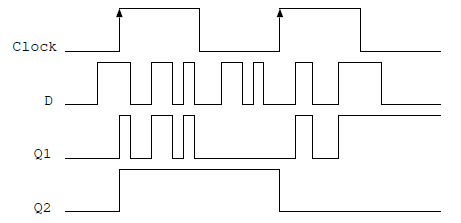
\includegraphics{assets/d_ff_timing.png}
	\caption{D-FFのタイミング図}
	\label{fig:d-ff_timing}
\end{figure}

\begin{figure}[H]
	\centering
	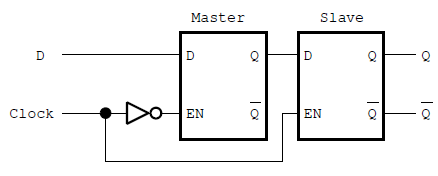
\includegraphics{assets/master_slave_d-ff.png}
	\caption{マスタスレーブ型D-FF}
	\label{fig:master_slave_d-ff}
\end{figure}

\subsubsection{有限状態機械}
有限状態機械は(FSM)は内部に有限個の状態(state)を持ち,その上で状態遷移規則を定義した機構である.
FSMの一種として,有限オートマトン(FA)や順序機械がある.

\subsubsection{カウンタ}
カウンタ(counter)はクロックに同期して値を加算(または減算)していく回路である.現在のカウント値を記憶するD-FFと,クロックごとに1加算する加算器を組み合わせて図\ref{fig:counter}のように構成する.
クロックの立ち上がりごとに現在のカウント値をインクリメントし,新しいカウント値をD-FFに記憶する.カウンタは値を数えるといった通常の用途の他,
クロック周波数を落とす目的や,回路内部の状態を記憶するためにも用いられる.
\begin{figure}
	\centering
	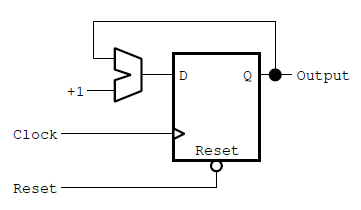
\includegraphics{assets/counter.png}
	\caption{カウンタの構造}
	\label{fig:counter}
\end{figure}

クロック周波数を落とす目的でカウンタを使用する場合は,カウンタの段数をいくつか増やしてClockを分周する.
各フリップフロップのクロック信号が共通ではない回路を非同期回路という.非同期カウンタでは,
カウンタの段数を増やすとそれぞれのカウンタで生じた遅延時間が累積し,最初段のカウンタと最後段のカウンタでは大きな時間差が生じることがある.
これに対し,共通のクロック信号ですべてのフリップフロップを駆動する回路を単相同期回路という.

\section{演習の解答}
\subsection{演習1}
4個のスライドスイッチで入力した4ビットの値を7セグメントディスプレイ1個に16進数1桁で表示する7セグメントデコーダモジュールを記述したソースコード\ref{src:7seg_decoder}を以下に示す.
また,出力信号とFPGAボードのピン名との対応を表\ref{tab:decoder-pin}に示す.なお,DE1-SoCのピン番号やピン名については参考文献\cite{user_manual}を参照した.
\begin{lstlisting}[caption=7セグメントデコーダモジュール, label=src:7seg_decoder]
module decoder_4x16 (D, Q);
	input [3:0] D;
	output [6:0] Q;
	reg [6:0] Q;
	
	always @(D) begin
		case (D)
			4'b0000: Q = 7'b1000000;
			4'b0001: Q = 7'b1111001;
			4'b0010: Q = 7'b0100100;
			4'b0011: Q = 7'b0110000;
			4'b0100: Q = 7'b0011001;
			4'b0101: Q = 7'b0010010;
			4'b0110: Q = 7'b0000010;
			4'b0111: Q = 7'b1011000;
			4'b1000: Q = 7'b0000000;
			4'b1001: Q = 7'b0010000;
			4'b1010: Q = 7'b0001000;
			4'b1011: Q = 7'b0000011;
			4'b1100: Q = 7'b1000110;
			4'b1101: Q = 7'b0100001;
			4'b1110: Q = 7'b0000110;
			4'b1111: Q = 7'b0001110;
			default: Q = 7'bxxxxxxx;
		endcase
	end
endmodule
\end{lstlisting}

\begin{table}[H]
	\centering
	\caption{出力信号とFPGAボードのピン名の対応}
	\begin{tabular}{|c|c|}
		\hline
		出力信号 & ピン名  \\ \hline
		Q[0]     & HEX0[0] \\ \hline
		Q[1]     & HEX0[1] \\ \hline
		Q[2]     & HEX0[2] \\ \hline
		Q[3]     & HEX0[3] \\ \hline
		Q[4]     & HEX0[4] \\ \hline
		Q[5]     & HEX0[5] \\ \hline
		Q[6]     & HEX0[6] \\ \hline
	\end{tabular}
	\label{tab:decoder-pin}
\end{table}

\subsection{演習2}
\subsubsection{T-FF}
T-FFのモジュールをソースコード\ref{src:t-ff}に示す.
\begin{lstlisting}[caption=T-FFのモジュール, label=src:t-ff]
module t_ff (Clk, T, Q, NQ);
	input Clk, T;
	output Q, NQ;
	reg Q, NQ;
	
	always @(posedge Clk) begin
		Q <= (T) ? ~Q : Q;
		NQ <= (T) ? Q : ~Q;
	end
endmodule
\end{lstlisting}

\subsubsection{JK-FF}
JK-FFのモジュールをソースコード\ref{src:jk-ff}に示す.
\begin{lstlisting}[caption=JK-FFのモジュール, label=src:jk-ff]
module jk_ff(Clk, J, K ,Q, NQ);
	input Clk, J, K;
	output Q, NQ;
	reg Q, NQ;
	
	always @(posedge Clk) begin
		case(J)
			1'b0: begin
				Q <= (K) ? 1'b0 : Q;
				NQ <= (K) ? 1'b1 : ~Q;
			end
			1'b1: begin
				Q <= (K) ? ~Q : 1'b1;
				NQ <= (K) ? Q : 1'b0;
			end
			default: begin
				Q <= 1'bx;
				NQ <= 1'bx;
			end
		endcase
	end
endmodule

\end{lstlisting}


\section{実習}
\subsection{実習1}
2ビット4-to-1マルチプレクサのモジュールをソースコード\ref{src:2bit_4to1_mux}に示す.
\begin{lstlisting}[caption=2ビット4-to-1マルチプレクサのモジュール, label=src:2bit_4to1_mux]
module mux_2bit_4to1(I0, I1, I2, I3, S, O);
	input [1:0] I0, I1, I2, I3, S;
	output [1:0] O;
	
	assign O = func_mux(I0, I1, I2, I3, S);
	
	function [1:0] func_mux;
		input [1:0] i0, i1, i2, i3, s;
		begin
			case (s)
				2'b00: func_mux = i0;
				2'b01: func_mux = i1;
				2'b10: func_mux = i2;
				2'b11: func_mux = i3;
				default: func_mux = 2'bxx;
			endcase
		end
	endfunction
endmodule 
\end{lstlisting}

次にソースコード\ref{src:2bit_4to1_mux}を用いたシミュレーション結果を図\ref{fig:result_mux_2bit_4to1}に示す.
シミュレーションでは,入力I0, I1, I2, I3の値をそれぞれ00, 01, 10, 11に設定している.
図\ref{fig:result_mux_2bit_4to1}から,Sの値を変えることで入力の選択が正しく行われ,正しい出力が得られることが分かる.
\begin{figure}[H]
	\centering
	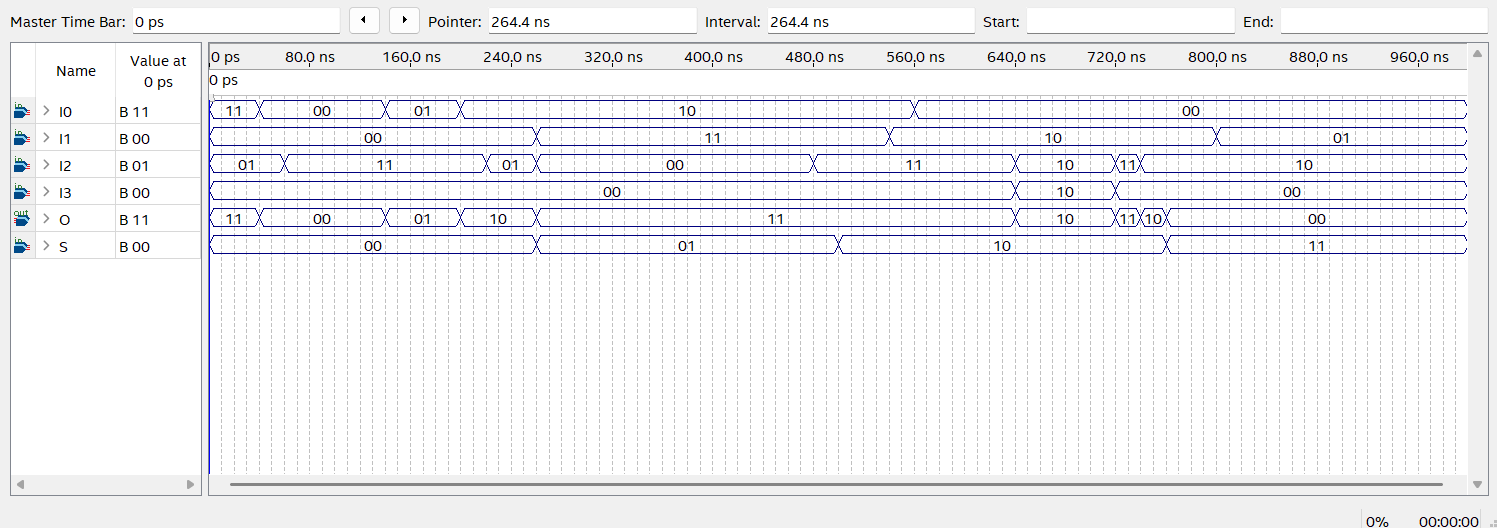
\includegraphics[width=\textwidth]{assets/mux_2bit_4to1_result_input_dif.png}
	\caption{2ビット4-to-1マルチプレクサのシミュレーション結果}
	\label{fig:result_mux_2bit_4to1}
\end{figure}

\subsection{実習2}
マスタスレーブ型D-FFのモジュールをソースコード\ref{src:master_slave_d-ff}に示す.
\begin{lstlisting}[caption=マスタスレーブ型D-FFのモジュール, label=src:master_slave_d-ff]
module d_ff_master_slave (Clk, D, Q);
	input Clk, D;
	output Q;
	wire q_m;
	
	d_latch M (~Clk, D, q_m);
	d_latch S (Clk, q_m, Q);
endmodule

module d_latch (EN, D, Q);
	input EN, D;
	output Q;
	reg Q;
	
	always @(EN or D)
		if (EN)
			Q <= D;	
endmodule
\end{lstlisting}

次に,ソースコード\ref{src:master_slave_d-ff}を用いたシミュレーション結果を図\ref{fig:result_master_slave_d-ff}に示す.
図\ref{fig:result_master_slave_d-ff}から,出力QがClockの立ち上がりのタイミングでのDの値を反映させていることがわかる.
これより,マスタスレーブ型D-FFが実装できていることが確認できる.
\begin{figure}
	\centering
	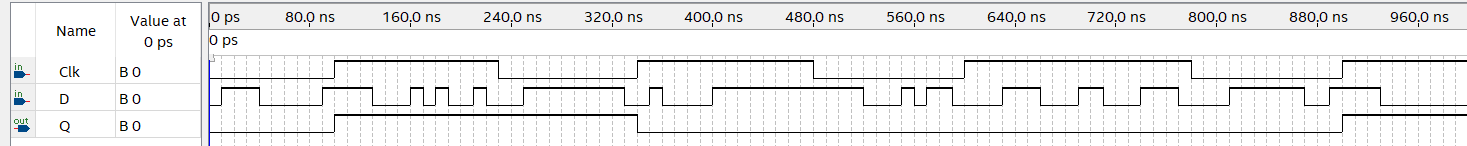
\includegraphics[width=\textwidth]{assets/dff_result.png}
	\caption{マスタスレーブ型D-FFのシミュレーション結果}
	\label{fig:result_master_slave_d-ff}
\end{figure}

\subsection{実習3}
設計した自動販売機の状態遷移図を図\ref{fig:state_transition_diagram}に示す.
\begin{figure}[H]
	\centering
	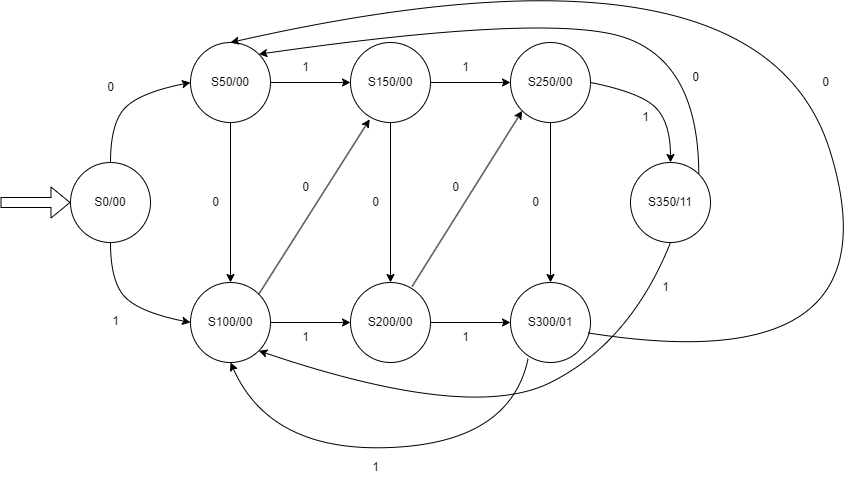
\includegraphics[width=0.9\textwidth]{assets/my_fsm.png}
	\caption{設計した自動販売機の状態遷移図}
	\label{fig:state_transition_diagram}
\end{figure}
図\ref{fig:state_transition_diagram}では,投入金額が0円でチケットや釣銭の出力が行われていない状態を初期状態S0/00としている.
また,自動販売機の入力イベントとして,50円投入したときが0,100円投入したときが1に対応している.
投入金額が300円になったときにチケットを出力(LEDR[0]が点灯)し,続けて硬貨を投入すれば,硬貨に応じてS50/00かS100/00に遷移する.
投入金額が350円になったときはチケットと釣銭を出力(LEDR[0]とLEDR[1]が点灯)し,続けて硬貨を投入すれば,同じように遷移する.

図\ref{fig:state_transition_diagram}をもとにVerilogで記述したモジュールをソースコード\ref{src:vending_machine}に示す.
\begin{lstlisting}[caption=状態遷移を行う自動販売機のモジュール, label=src:vending_machine]
module vending_machine(Clk, I, Resetn, Q);
	input Clk, I, Resetn;
	output [1:0] Q;
	
	parameter  S0 = 3'b000,
				 S50 = 3'b001,
				 S100 = 3'b010,
				 S150 = 3'b011,
				 S200 = 3'b100,
				 S250 = 3'b101,
				 S300 = 3'b110,
				 S350 = 3'b111; 
	reg [2:0] cur_st, next_st;
	
	assign Q = 
		(cur_st == S300) ? 2'b01 : (
		(cur_st == S350) ? 2'b11 : 2'b00);
				  
	always @(posedge Clk)
		if(!Resetn)
			cur_st <= S0;
		else
			cur_st <= next_st;
	
	always @(cur_st or I)
		case(cur_st)
			S0	   : next_st = (I) ? S100 : S50;
			S50    : next_st = (I) ? S150 : S100;
			S100   : next_st = (I) ? S200 : S150;
			S150   : next_st = (I) ? S250 : S200;
			S200   : next_st = (I) ? S300 : S250;
			S250   : next_st = (I) ? S350 : S300;
			S300   : next_st = (I) ? S100 : S50;
			S350   : next_st = (I) ? S100 : S50;
			default: next_st = 3'bxxx;
		endcase
endmodule
\end{lstlisting}

次に,ソースコード\ref{src:vending_machine}から,State Machine Viewerで表示した状態遷移図を図\ref{fig:state_machine_viewer_output}に示す.
また,このときの遷移条件の表を表\ref{tab:state_transition_table}に示す.なお,表\ref{tab:state_transition_table}にあるIの値は,
硬貨の種類に対応しており,I = 0のときは50円が投入された,I = 1のときは100円が投入されたことを意味している.
\begin{figure}[H]
	\centering
	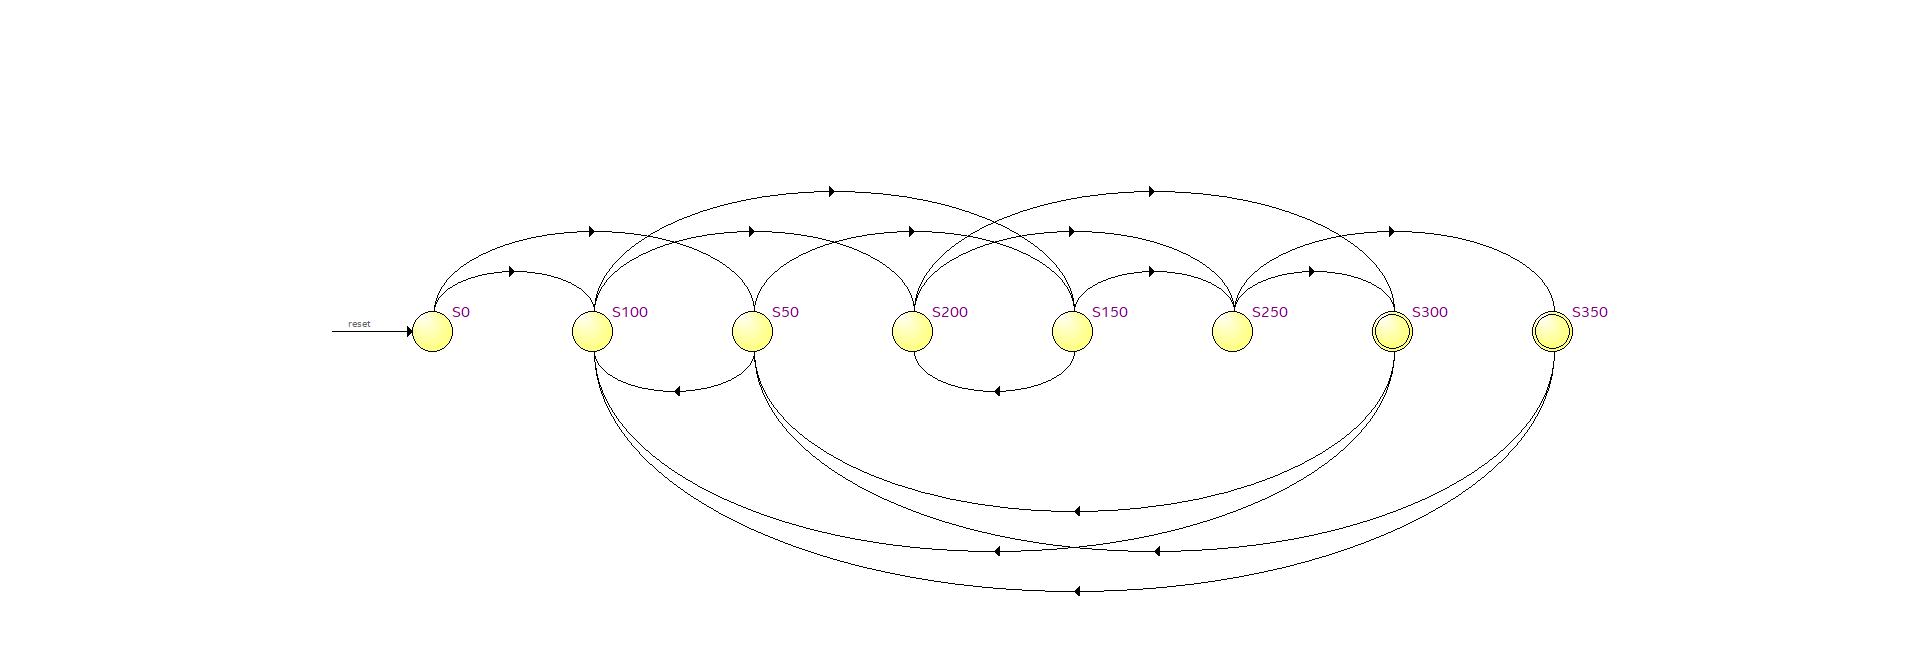
\includegraphics[width=\textwidth]{assets/vending_machine_state_viewer.png}
	\caption{State Machine Viewerで表示した状態遷移図}
	\label{fig:state_machine_viewer_output}
\end{figure}

\begin{table}[H]
	\centering
	\caption{図\ref{fig:state_machine_viewer_output}の状態遷移条件}
	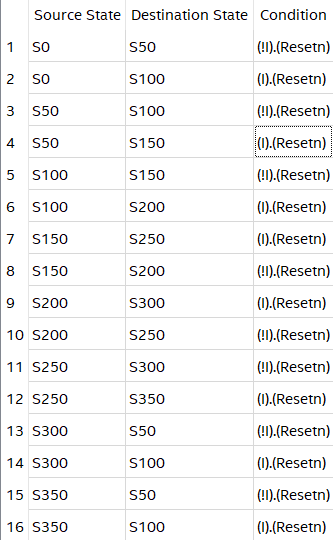
\includegraphics{assets/state_transition_table.png}
	\label{tab:state_transition_table}
\end{table}

図\ref{fig:state_transition_diagram}と図\ref{fig:state_machine_viewer_output}を比較すると,状態の配置の仕方は異なるが,
表\ref{tab:state_transition_table}から遷移条件が設計通りに反映されていることが分かる.したがって,コードが正しく実装されていることが確認できる.

ソースコード\ref{src:vending_machine}をもとに行ったシミュレーション結果を図\ref{fig:vending_machine_sim}に示す.
\begin{figure}[H]
	\centering
	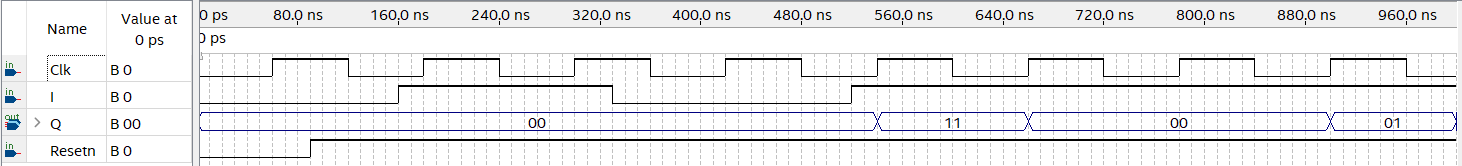
\includegraphics[width=\textwidth]{assets/vending_machine_sim.png}
	\caption{ソースコード\ref{src:vending_machine}のシミュレーション結果}
	\label{fig:vending_machine_sim}
\end{figure}

図\ref{fig:vending_machine_sim}において,Clockが立ち上がるときのIの値を見ると,1回目の立ち上がり時はResetnが0に指定されているため加算されない.
2,3回目の立ち上がりではI=1となっているため100円が投入され,4回目の立ち上がりではI=0となっているため50円が投入されている.
5回目の立ち上がり時はI=1となっているため100円が投入されており,ここで投入金額が350円になる.また,図\ref{fig:vending_machine_sim}より出力がQ=11となっているため,
チケットと釣銭の出力が行われていることが確認できる.続いて6,7,8回目の立ち上がりではそれぞれI=1となっているため100円が投入されている.
8回目の立ち上がり時に投入金額が300円となるが,図\ref{fig:vending_machine_sim}を見ると,チケットの出力がきちんと行われている(Q=01)ことが確認できる.

実習3については実機実験を行う予定であったが,時間が足りなかったため実機実験を行えなかった.
そのため,実機に書き込めるように準備しておいた状態で,実験はシミュレーション上で行った.

\subsection{実習4}
PWM制御により,赤色LEDの輝度を調節する回路をVerilog HDLで記述したものをソースコードに示す.
\begin{lstlisting}[caption=赤色LEDの輝度を調節するモジュール, label=src:led_adjust]
module pwm(Clk, I, Resetn, Q);
	input Clk, Resetn;
	input [7:0] I;
	output wire Q;
	reg [7:0] Count;
	
	assign Q = (Count < I) ? 1 : 0;
	
	always @(posedge Clk or negedge Resetn)
	begin
		if(!Resetn)
			Count <= 8'h00;
		else
			if(Count >= 8'hFF)
				Count <= 8'h00;
			else
				Count <= Count + 1'b1;
	end
endmodule
\end{lstlisting}

ソースコード\ref{src:led_adjust}からRTL Viewerで作成した回路を図\ref{fig:pwm_rtl_viewer}に示す.
\begin{figure}[H]
	\centering
	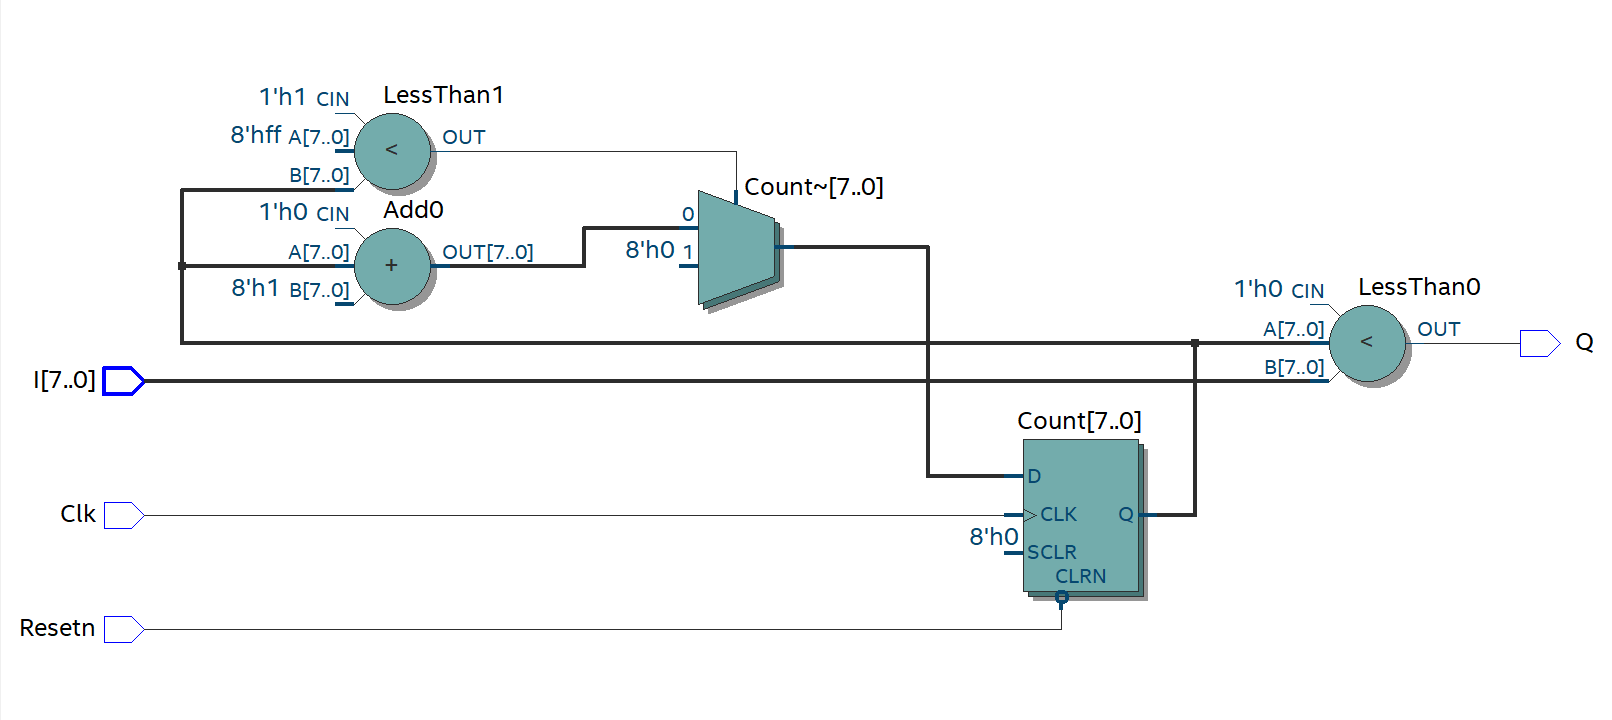
\includegraphics[width=\textwidth]{assets/pwm_rtl_viewer.png}
	\caption{RTL Viewerで作成した回路}
	\label{fig:pwm_rtl_viewer}
\end{figure}

次に,実際の回路の動作を確認する.ただし,時間の都合上実機実験は行えなかったため,実験はシミュレーション上で行う.
シミュレーションの結果を図\ref{fig:result_pwm_255}~\ref{fig:result_pwm_0}に示す.なお,クロックの周期は1nsとした.
\begin{figure}[H]
	\centering
	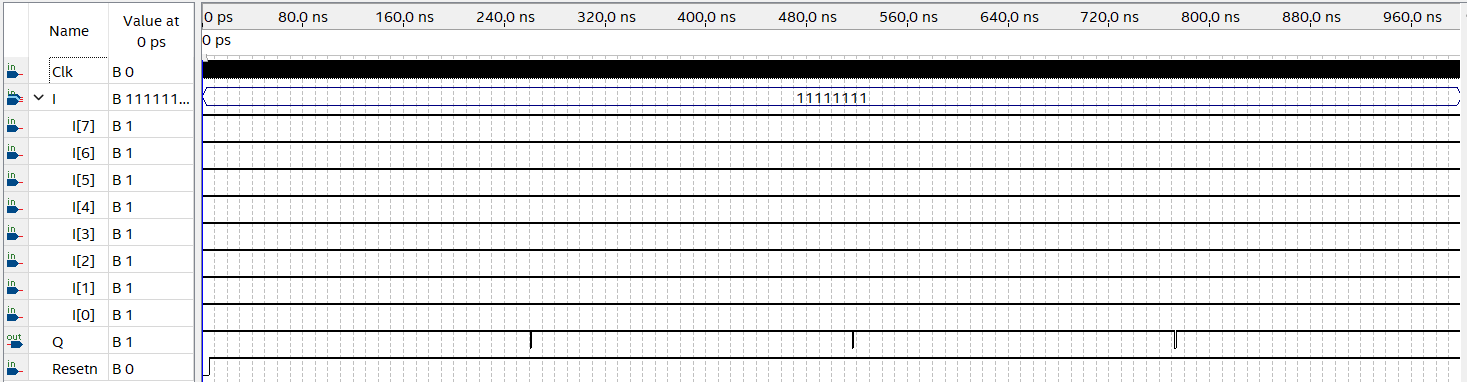
\includegraphics[width=\textwidth]{assets/pwm_255_1ns.png}
	\caption{輝度255(I = 11111111)のときのシミュレーション結果}
	\label{fig:result_pwm_255}
\end{figure}
\begin{figure}[H]
	\centering
	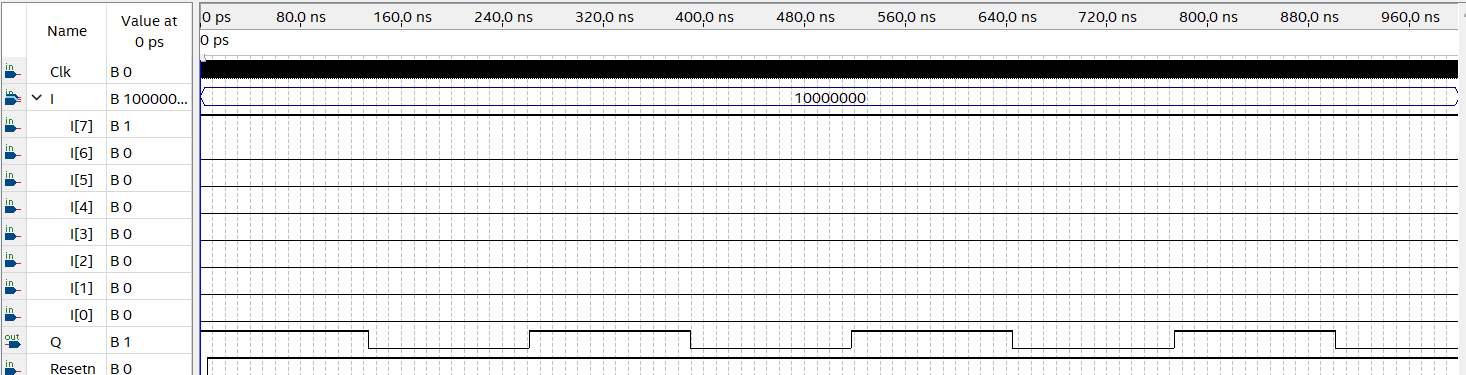
\includegraphics[width=\textwidth]{assets/pwm_128_1ns.png}
	\caption{輝度128(I = 10000000)のときのシミュレーション結果}
	\label{fig:result_pwm_128}
\end{figure}
\begin{figure}[H]
	\centering
	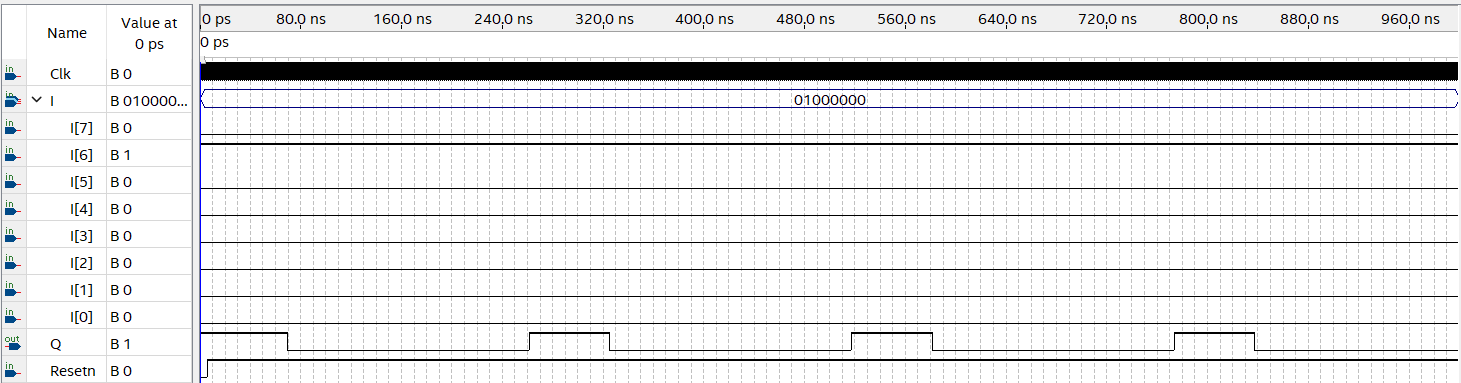
\includegraphics[width=\textwidth]{assets/pwm_64_1ns.png}
	\caption{輝度64(I = 01000000)のときのシミュレーション結果}
	\label{fig:result_pwm_64}
\end{figure}
\begin{figure}[H]
	\centering
	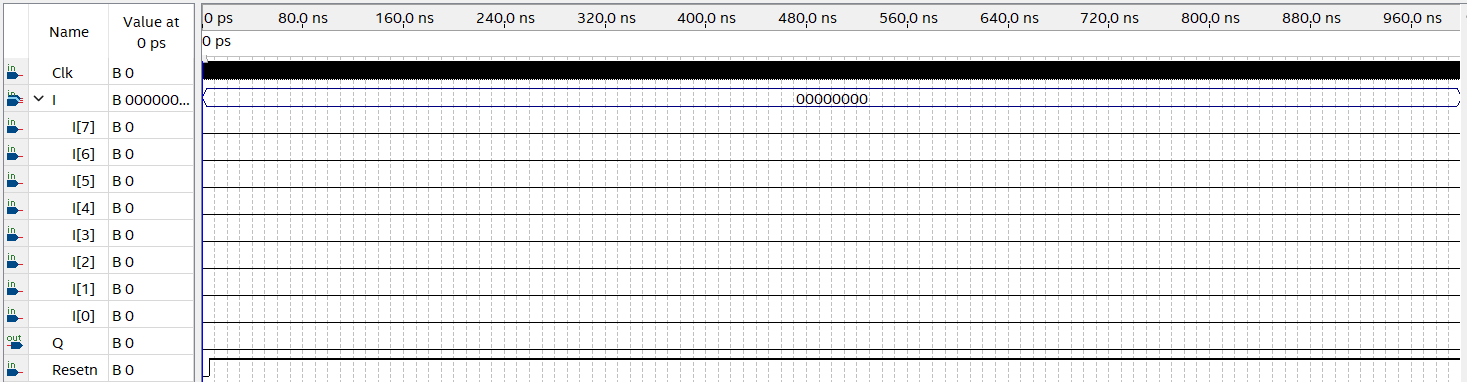
\includegraphics[width=\textwidth]{assets/pwm_0_1ns.png}
	\caption{輝度0(I = 00000000)のときのシミュレーション結果}
	\label{fig:result_pwm_0}
\end{figure}

図\ref{fig:result_pwm_255}~\ref{fig:result_pwm_0}から分かる通り,輝度が小さくなるにつれてデューティー比も小さくなっている.
また,図\ref{fig:result_pwm_128}と図\ref{fig:result_pwm_64}より,輝度が半分になるとパルス幅も半分になっていることが分かる.
図\ref{fig:result_pwm_0}より,輝度が0の時は出力Qが0のまま一定となり,LEDが点灯しないと考えられる.
以上より,PWM制御でのLEDの輝度調整の動作が正しいことが確認できた.

\section{考察}
HDLを用いたハードウェアの記述と,ソースコードを反映させたシミュレータの利用方法を身に着けることができた.
PWM制御を行うモジュールの記述ではカウンタを利用することで輝度などの表現ができることを理解した.
また,今回は実機実験での動作確認が行えなかったが,シミュレーションの結果が設計通りであることと,信号とFPGAボードの
ピンを対応させることが問題なくできることから,実機実験でも問題なく動作する可能性が高い.

\begin{thebibliography}{9}
	\bibitem{exp_text} 布目 淳.プロジェクト実習Ⅲ 論理設計 実験テキスト.京都工芸繊維大学,2024年
	\bibitem{user_manual} Terasic Technologics Inc.:  ``DE1-SoC User Manual V2.0.4'' Chapter3. Using the DE1-SoC Board, 2019
\end{thebibliography}

\end{document}